% Für Bindekorrektur als optionales Argument "BCORfaktormitmaßeinheit", dann
% sieht auch Option "twoside" vernünftig aus
% Näheres zu "scrartcl" bzw. "scrreprt" und "scrbook" siehe KOMA-Skript Doku
\documentclass[12pt,a4paper,titlepage,headinclude,bibtotoc]{scrartcl}


%---- Allgemeine Layout Einstellungen ------------------------------------------

% Für Kopf und Fußzeilen, siehe auch KOMA-Skript Doku
\usepackage[komastyle]{scrpage2}
\pagestyle{scrheadings}
\automark[section]{chapter}
\setheadsepline{0.5pt}[\color{black}]

%keine Einrückung
\parindent0pt

%Einstellungen für Figuren- und Tabellenbeschriftungen
\setkomafont{captionlabel}{\sffamily\bfseries}
\setcapindent{0em}

\usepackage{caption}

%---- Weitere Pakete -----------------------------------------------------------
% Die Pakete sind alle in der TeX Live Distribution enthalten. Wichtige Adressen
% www.ctan.org, www.dante.de

% Sprachunterstützung
\usepackage[ngerman]{babel}

% Benutzung von Umlauten direkt im Text
% entweder "latin1" oder "utf8"
\usepackage[utf8]{inputenc}

% Pakete mit Mathesymbolen und zur Beseitigung von Schwächen der Mathe-Umgebung
\usepackage{latexsym,exscale,amssymb,amsmath}

% Weitere Symbole
\usepackage[nointegrals]{wasysym}
\usepackage{eurosym}

% Anderes Literaturverzeichnisformat
%\usepackage[square,sort&compress]{natbib}

% Für Farbe
\usepackage{color}

% Zur Graphikausgabe
%Beipiel: \includegraphics[width=\textwidth]{grafik.png}
\usepackage{graphicx}

% Text umfließt Graphiken und Tabellen
% Beispiel:
% \begin{wrapfigure}[Zeilenanzahl]{"l" oder "r"}{breite}
%   \centering
%   \includegraphics[width=...]{grafik}
%   \caption{Beschriftung} 
%   \label{fig:grafik}
% \end{wrapfigure}
\usepackage{wrapfig}

% Mehrere Abbildungen nebeneinander
% Beispiel:
% \begin{figure}[htb]
%   \centering
%   \subfigure[Beschriftung 1\label{fig:label1}]
%   {\includegraphics[width=0.49\textwidth]{grafik1}}
%   \hfill
%   \subfigure[Beschriftung 2\label{fig:label2}]
%   {\includegraphics[width=0.49\textwidth]{grafik2}}
%   \caption{Beschriftung allgemein}
%   \label{fig:label-gesamt}
% \end{figure}
\usepackage{subfigure}
\usepackage{adjustbox}

% Caption neben Abbildung
% Beispiel:
% \sidecaptionvpos{figure}{"c" oder "t" oder "b"}
% \begin{SCfigure}[rel. Breite (normalerweise = 1)][hbt]
%   \centering
%   \includegraphics[width=0.5\textwidth]{grafik.png}
%   \caption{Beschreibung}
%   \label{fig:}
% \end{SCfigure}
\usepackage{sidecap}

% Befehl für "Entspricht"-Zeichen
\newcommand{\corresponds}{\ensuremath{\mathrel{\widehat{=}}}}

%Für chemische Formeln (von www.dante.de)
%% Anpassung an LaTeX(2e) von Bernd Raichle
\makeatletter
\DeclareRobustCommand{\chemical}[1]{%
  {\(\m@th
   \edef\resetfontdimens{\noexpand\)%
       \fontdimen16\textfont2=\the\fontdimen16\textfont2
       \fontdimen17\textfont2=\the\fontdimen17\textfont2\relax}%
   \fontdimen16\textfont2=2.7pt \fontdimen17\textfont2=2.7pt
   \mathrm{#1}%
   \resetfontdimens}}
\makeatother

%Si Einheiten
\usepackage{siunitx}

%c++ Code einbinden
\usepackage{listings}
\lstset{numbers=left, numberstyle=\tiny, numbersep=5pt}

%Differential
\newcommand{\dif}{\ensuremath{\mathrm{d}}}

%Boxen,etc.
\usepackage{fancybox}
\usepackage{empheq}

%Fußnoten auf gleiche Seite
\interfootnotelinepenalty=1000

%Dateien aus Unterverzeichnissen
\usepackage{import}

%Bibliography \bibliography{literatur} und \cite{gerthsen}
%\usepackage{cite}
\usepackage{babelbib}
\selectbiblanguage{ngerman}

\begin{document}

\begin{titlepage}
\centering
\textsc{\Large Anfängerpraktikum der Fakultät für
  Physik,\\[1.5ex] Universität Göttingen}

\vspace*{4.2cm}

\rule{\textwidth}{1pt}\\[0.5cm]
{\huge \bfseries
  Das Prismen- und\\[1.5ex]
  Gitterspektrometer}\\[0.5cm]
\rule{\textwidth}{1pt}

\vspace*{3.0cm}

\begin{Large}
\begin{tabular}{ll}
Praktikant:
 	&  Felix Kurtz\\
 	&  Michael Lohmann\\

E-Mail: 
	&  felix.kurtz@stud.uni-goettingen.de\\
	& m.lohmann@stud.uni-goettingen.de\\

 Betreuer: & Phillip Batian\\
 Versuchsdatum: &  05.03.2015\\
\end{tabular}
\end{Large}

\vspace*{0.8cm}

\begin{Large}
\fbox{
  \begin{minipage}[t][2.5cm][t]{6cm} 
    Testat:
  \end{minipage}
}
\end{Large}

\end{titlepage}

\tableofcontents

\newpage

\section{Einleitung}
\label{sec:einleitung}
Mit einem Gitter kann man durch Interferenzeffekte weißes Licht in seine Spektralfarben zerlegt werden.
Das Gleiche kann man auch auf Grund der Dispersion mit einem Prisma tun.
In diesem Versuch sollen an einer Quecksilber-Dampflampe beide Verfahren  bezüglich des Auflösungsvermögens verglichen werden.

\section{Theorie}
\label{sec:theorie}
\subsection{Prismenspektrometer}

\begin{figure}[!h]
	\centering
	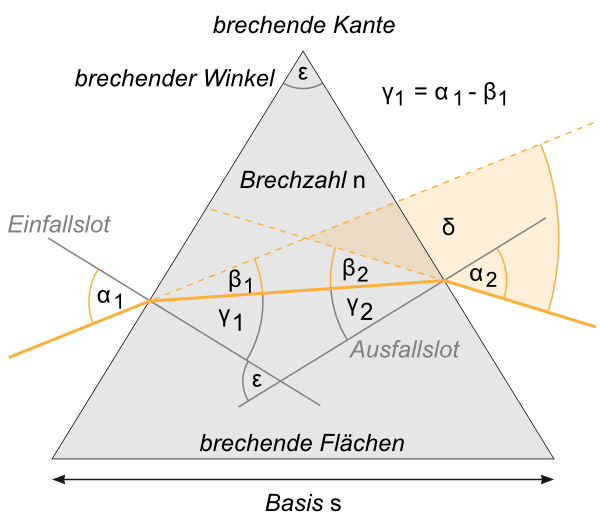
\includegraphics[scale=0.6]{Prisma.png}
	\caption{Prismaquerschnitt mit Strahlengang. \cite[Datum: 28.12.2014]{LP19}}
	\label{fig:prisma}
\end{figure}
Dieses Spektrometer basiert auf der \textit{Dispersion}, also der Wellenlängenabhängigkeit des Brechungsindex.
Unter \textit{normaler} Dispersion versteht man, dass der Brechungsindex $n$ mit zunehmender Wellenlänge abnimmt.
Bei anomaler Dispersion geschieht das Gegenteil: $\frac{\dif n}{\dif \lambda} > 0$.\\

Snellius'sches Brechungsgesetz $n_1\cdot\sin\alpha_1=n_2\cdot\sin\alpha_2$\\

Mit dem Brechungsgesetz  und den geometrischen Beziehungen aus Abb.\ref{fig:prisma} $\gamma_1+\gamma_2=\varepsilon$ sowie $\delta=\alpha_1+\alpha_2-\epsilon$ folgt bei symmetrischer Durchstrahlung ($\alpha_1=\alpha_2$) für den Ablenkwinkel $\delta_\text{min}$, der so minimal wird,

\begin{align}
	\sin\left(\frac{\delta_\text{min}+\varepsilon}{2}\right)=n\cdot\sin\left(\frac{\varepsilon}{2}\right)\,.
\end{align}

Leitet man diese Beziehung nach $n$ ab

\begin{align}
	\cos\left(\frac{\delta_\text{min}+\varepsilon}{2}\right)\cdot \frac{\dif \delta}{\dif n}=\sin\left(\frac{\varepsilon}{2}\right)
\end{align}

\begin{figure}[!h]
	\centering
	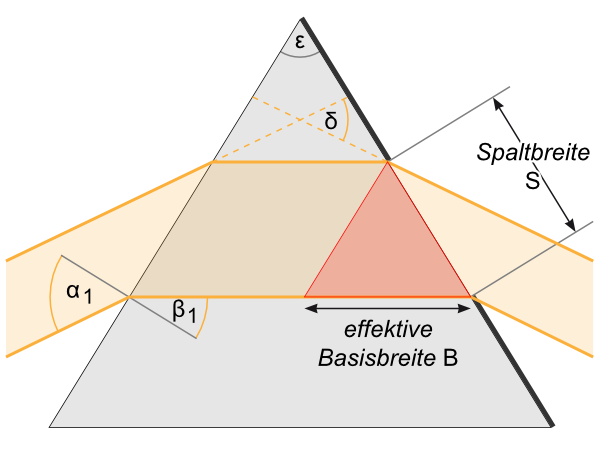
\includegraphics[scale=0.6]{Prisma2.png}
	\caption{Skizze zur Bestimmung des Auflösungsvermögens. \cite[Datum: 28.12.2014]{LP19}}
	\label{fig:prisma2}
\end{figure}

\begin{align}
	\frac{\dif \delta}{\dif n}=\frac{B}{S}
\end{align}

\textbf{Auflösungsvermögen} $A:=\frac{\lambda}{\Delta\lambda}$

\begin{align}
	A=B\left|\frac{\dif n}{\dif \lambda}\right|
\end{align}

\subsection{Gitterspektrometer}
\begin{align}
	\sin\alpha_\text{max}&=\frac{k\lambda}{a}\\
	\sin\alpha_\text{min}&=\frac{n\lambda}{Na}
\end{align}

Somit ist das Auflösungsvermögen durch
\begin{align}
	A=kN
\end{align}
gegeben.

\subsection{Quecksilber-Dampflampe}

\section{Durchführung}
\label{sec:durchfuehrung}

\begin{figure}[!h]
	\centering
	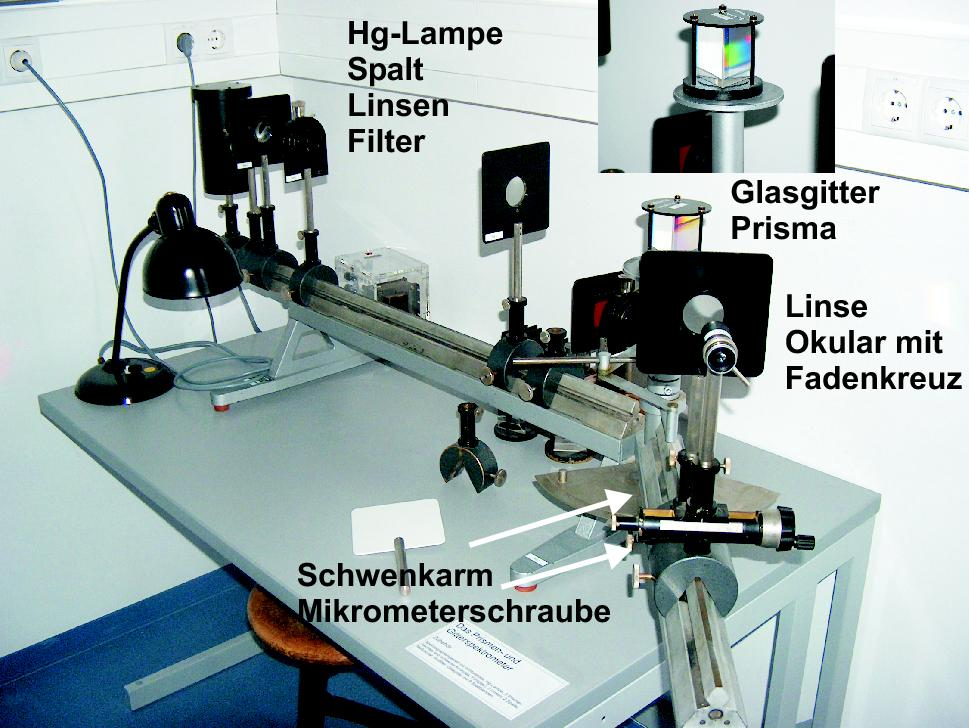
\includegraphics[scale=0.4]{Aufbau.jpg}
	\caption{Der Versuchsaufbau. \cite[Datum: 28.12.2014]{LP19}}
	\label{fig:aufbau}
\end{figure}

\subsection{Prismenspektrometer}
Folgende Schritte werden zuerst mit dem Kronglas-Prisma durchgeführt, danach mit dem Prisma aus schwerem Flintglas.
Bei beiden misst man die geometrischen Basislängen.\\

Zuerst wird der Spektralapparat aufgebaut und justiert.
Dazu werden die Hg-Lampe, die Kondensorlinse, der Beleuchtungsspalt sowie die zweite Linse in der gleichen Reihenfolge wie in Abb. \ref{fig:aufbau} befestigt - und zwar so, dass die Lichtstrahlen danach parallel sind.
Mit der dritten Linse und dem Okular wird der Spalt scharf abgebildet.
Zur späteren Auswertung werden die Brennweiten und Linsenpositionen notiert.
Nun wird das Fadenkreuz des Okulars auf den Strahl eingestellt und die Position der Winkelskala sowie des Feintriebs notiert.

Danach wird das Prisma in den Strahlengang gestellt und so gedreht, dass das Prisma symmetrisch durchstrahlt wird (minimaler Ablenkwinkel).
Der Schwenkarm wird nun auf eine der gelben Linien justiert.
Den Winkel notiert man.

Über den Abstand der eingestellten gelben Linie zur grünen Linie (Feintrieb des Okulars, der Schwenkarm wird nicht verstellt) und den Abstand der dritten Linse zum Okular kann der Ablenkwinkel $\Delta\varphi$ zwischen den beiden Linien bestimmt werden.

Nun verengt man den Strahl mit einem zweiten Spalt vor dem Prisma gerade so, dass die beiden gelben Linien noch getrennt erscheinen.
Dieser Spalt ersetzt nun den Eingangsspalt, das Prisma wird entfernt und durch den Rotfilter ersetzt, der Schwenkarm wird zurückgeschwenkt.
Mit dem Messokular vermisst man nun das Spaltbild.

\subsection{Gitterspektrometer}
Nun benutzt man das Glasgitter, welches sehr empfindlich ist und nicht berührt werden darf.

Der Aufbau ist der gleiche wie im obigen Abschnitt.
Es wird lediglich das Gitter anstelle des Prismas gesetzt -- möglichst senkrecht zum Strahl.
Für die erste, vierte und achte Ordnung werden die Ablenkwinkel der grünen Linie sowie der gelben und violetten Doppellinien bestimmt.

Für die 1., 4. und 8. Ordnung der beiden gelben Linien wird in die Plexiglasführung nacheinander kleinere Spaltblenden eingeführt und so die Blende $d_\text{min}$ bestimmt, so dass die beiden Linien gerade nicht mehr getrennt aufgelöst werden.

\section{Auswertung}
\label{sec:auswertung}


\section{Diskussion}
\label{sec:diskussion}

\section{Anhang}

\bibliography{literatur}
\bibliographystyle{babalpha}

\end{document}
